\newpage
\section{Auswertung}

Um die aufgenommenen Daten zu analysieren werden die Python~\cite{python} Pakete NumPy~\cite{numpy} und SciPy~\cite{scipy} verwendet,
wobei Matplotlib~\cite{matplotlib} zum Erstellen von Grafiken und zudem Uncertainties~\cite{uncertainties} zur automatisierten
Fehlerfortpflanzung in linearer Ordnung dienen.



\subsection{Verzögerungszeit}

\begin{figure}[H]
	\centering
	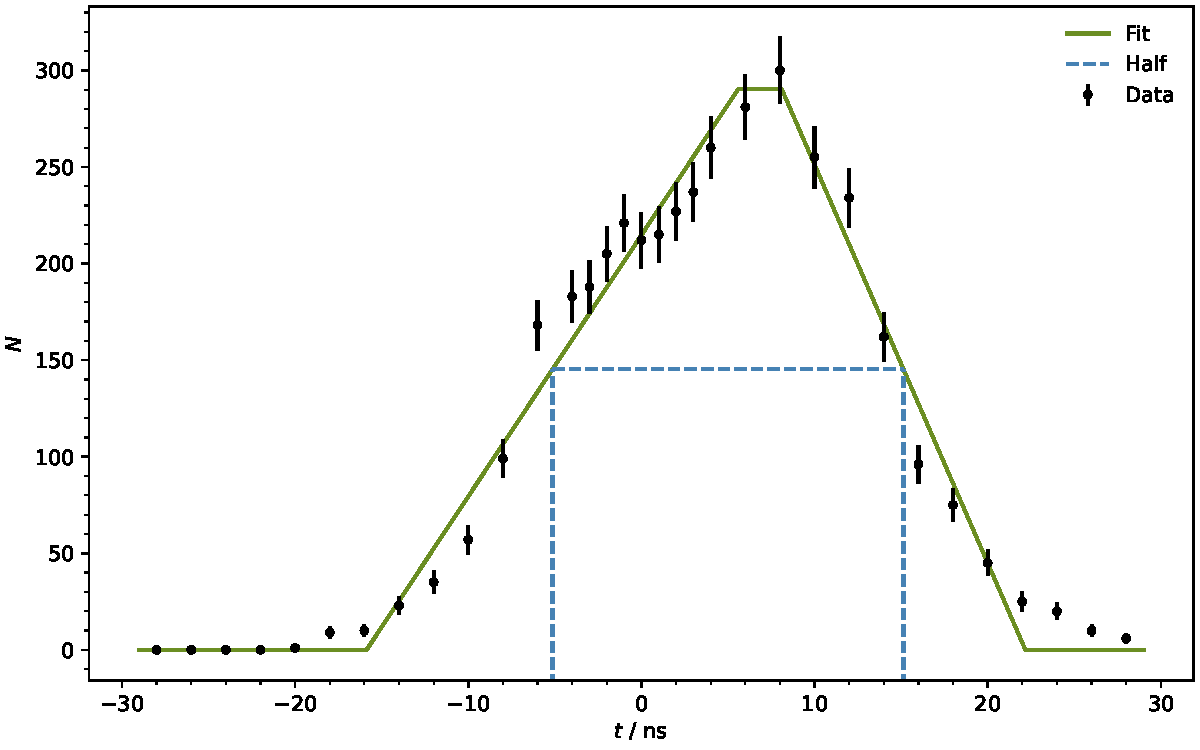
\includegraphics[width=\textwidth]{build/delay.pdf}
	\caption{.}
	\label{fig:delay}
\end{figure}



\subsection{Kanalkalibration}

\begin{figure}[H]
	\centering
	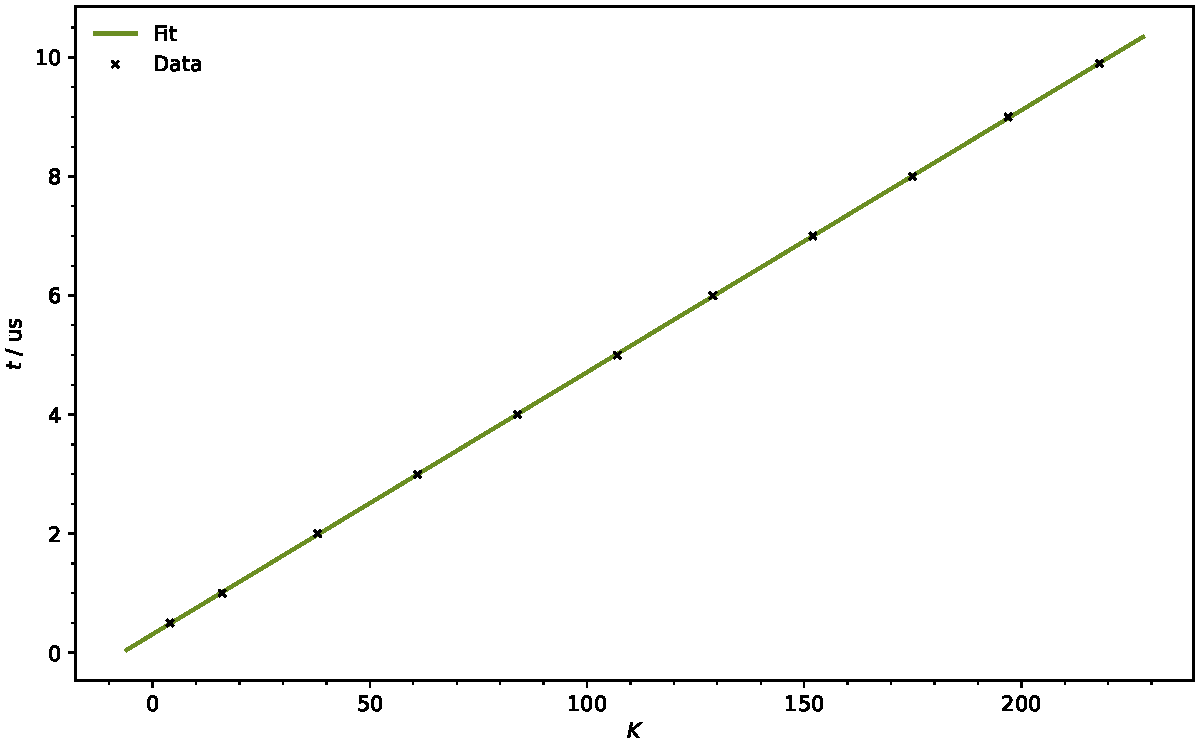
\includegraphics[width=\textwidth]{build/calibration.pdf}
	\caption{.}
	\label{fig:calibration}
\end{figure}



\subsection{Langzeitmessung}

\begin{figure}[H]
	\centering
	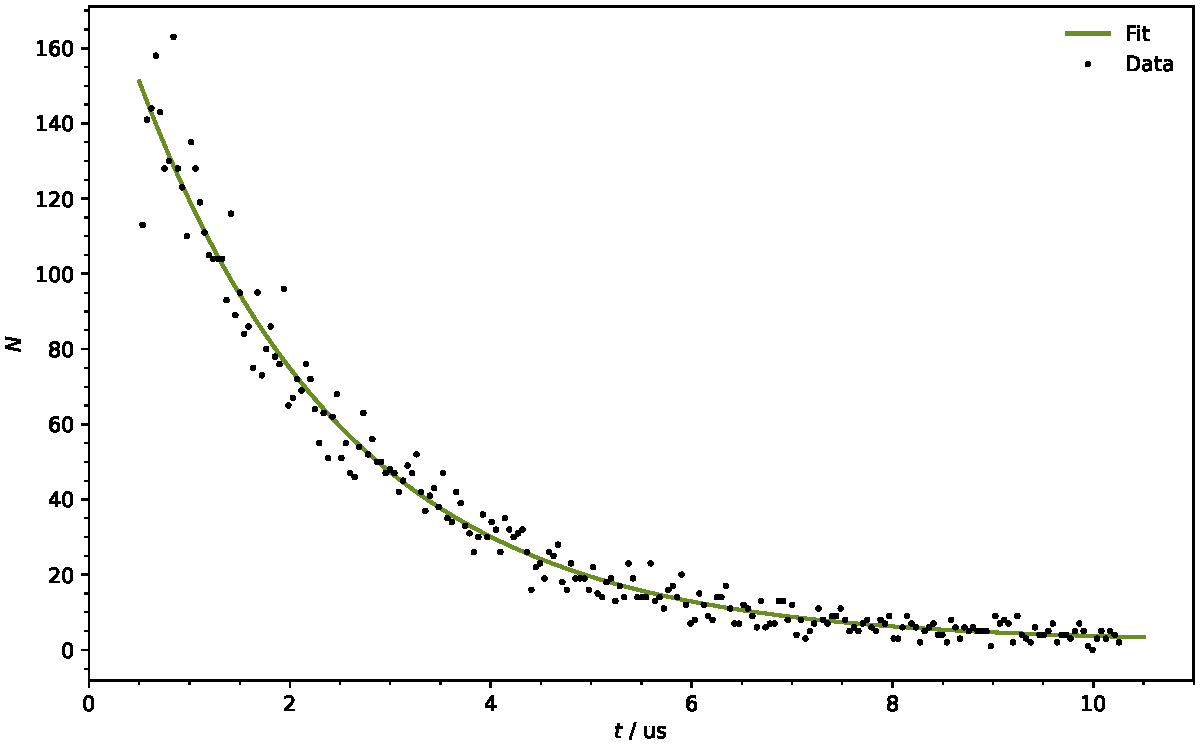
\includegraphics[width=\textwidth]{build/lifetime.pdf}
	\caption{.}
	\label{fig:lifetime}
\end{figure}



\subsection{Hintergrundrate}
